\section{Results}
\label{sec:Results}

\fix{Nathan and Ron}

\subsection{Experimental Setup}

All experiments were performed on the Cielo supercomputer housed at Los Alamos
National Laboratory.  Cielo is an 1,840-node Cray XE6 resource for the Advanced
Simulation and Computing (ASC) program and is jointly managed by Sandia National 
Laboratories and Los Alamos National Laboratories under the New Mexico
Alliance for Computing at Extreme Scale (ACES) project.  Each node contains
two AMD Opteron 6100 (Magny-Cours) 8-way processor chips for a total of 16 cores
per node.  Each core has a peak computational speed of 2.6 GHz, leading to a total 
theoretical peak of 1.37 Petaflops for the machine. The compute nodes each
have 32 GB of memory.  The interconnect consists of a proprietary Cray Gemini
Network with a 3D Torus topology and has a peak throughput rate of 6 GB/s/link. 

The experiments in this report include strong scaling results for four different
CTH applications: an application that writes spyplot files, representing the traditional 
post-processing approach; an application that uses a Nessie servivce to provide in-transit
ParaView analysis; and two applications that perform ParaView in-situ analysis.  The first 
in-situ application, labeled \emph{in-situ (untuned)}, uses an algorithm that does not scale.
The second in-situ application, labeled \emph{in-situ (tuned)}, uses a more
scalable implementation of the same algorithm.  

%%%%%%%%%%%%%%%%%%%%%% -- table ---
\begin{table}

\caption{Scaling Overview}
\label{tab:ScalingOverview}

\centering{}%
\begin{tabular}{|c|c|c|}
\hline 
Data Set Size (blocks) & Client Ranks (16 cores/node) & Server Nodes (2, 4, and 8 cores/node)\tabularnewline
\hline 
\hline 
33k & 128, 256, 512, 1024 & 2\tabularnewline
\hline 
220k & 1024, 2048, 4096, 8192 & 16\tabularnewline
\hline 
1.5m & 4096, 8192, 16384, 32768 & 128\tabularnewline
\hline 
\end{tabular}
\end{table}

%%%%%%%%%%%%%%%%%%%%%% -- table ---

For each application, we run strong scaling experiments for three different datasets.  
Table~\ref{tab:ScalingOvewview} shows the range of core sizes used for the various
experiments.  The objective is run experiments with datasets representative of real
production runs.  The number of nodes/cores used is limited by amount of memory required
for a particular experiment.  


NEED MORE... WILL FINISH TOMORROW


\subsection{Total Runtime Measurements}


\subsection{Per Cycle Timings}





The following plots provide measured values of total runtime for each of the 

Total runtime is the ultimate measure of the performance when comparing 
approaches.  


\subsection{Memory}
The following memory plots were taken by examining free memory on the nodes
using /proc/meminfo.  Measuring free memory is conservative because it also
accounts for caches and buffers, so although you may run out of free memory in
a system, the execution will not immediately fail due to memory freed from
those other sources.  However, these are an indication of the worst case
possible.  On Cielo there are 16 cores per node and in each case the nodes were
 loaded with 16 MPI ranks executing the statically linked executable.  

In order to understand CTH memory usage results, it is important to note that
CTH preallocates memory based on a value for "max number of blocks" provided
through the input deck.  Because of this, CTH memory usage is highly impacted
by the user specification.  In this case we ran the results with what we
believe are reasonable values for "max number of blocks" given the size of the
problem.  Figure~\ref{fig:MaxBlocks} shows the corresponding max blocks for
each run.

\begin{figure}[htb]
  \centering
  \includegraphics[width=\linewidth]{figures/MemoryUsageInSituPerNode.pdf}
  \caption{Plot of average per node memory usage of the in-situ run on Cielo.}
  \label{fig:MemoryInSituPerNode}
\end{figure}

\begin{figure}[htb]
  \centering
  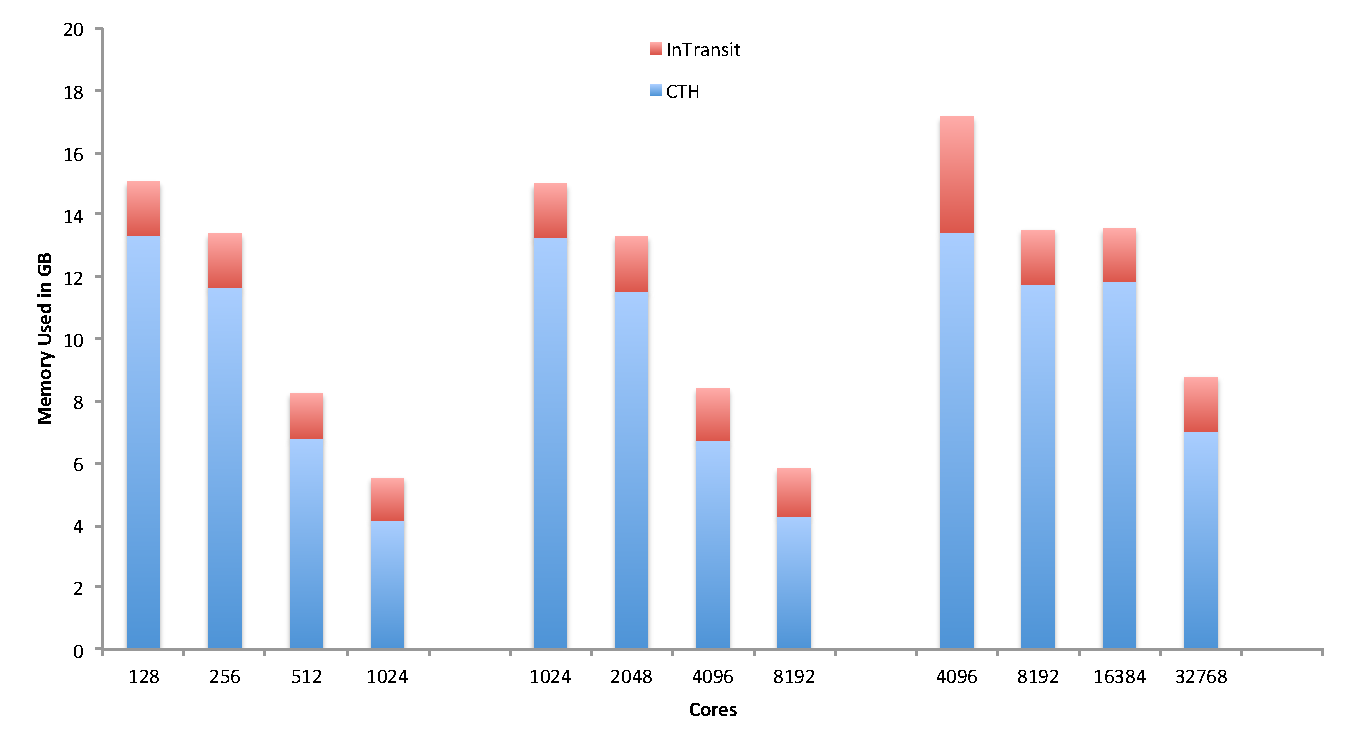
\includegraphics[width=\linewidth]{figures/MemoryUsageInTransitPerNode.pdf}
  \caption{Plot of average per node memory usage of the in-transit run on Cielo.}
  \label{fig:MemoryInTransitPerNode}
\end{figure}

\begin{figure}[htb]
  \centering
  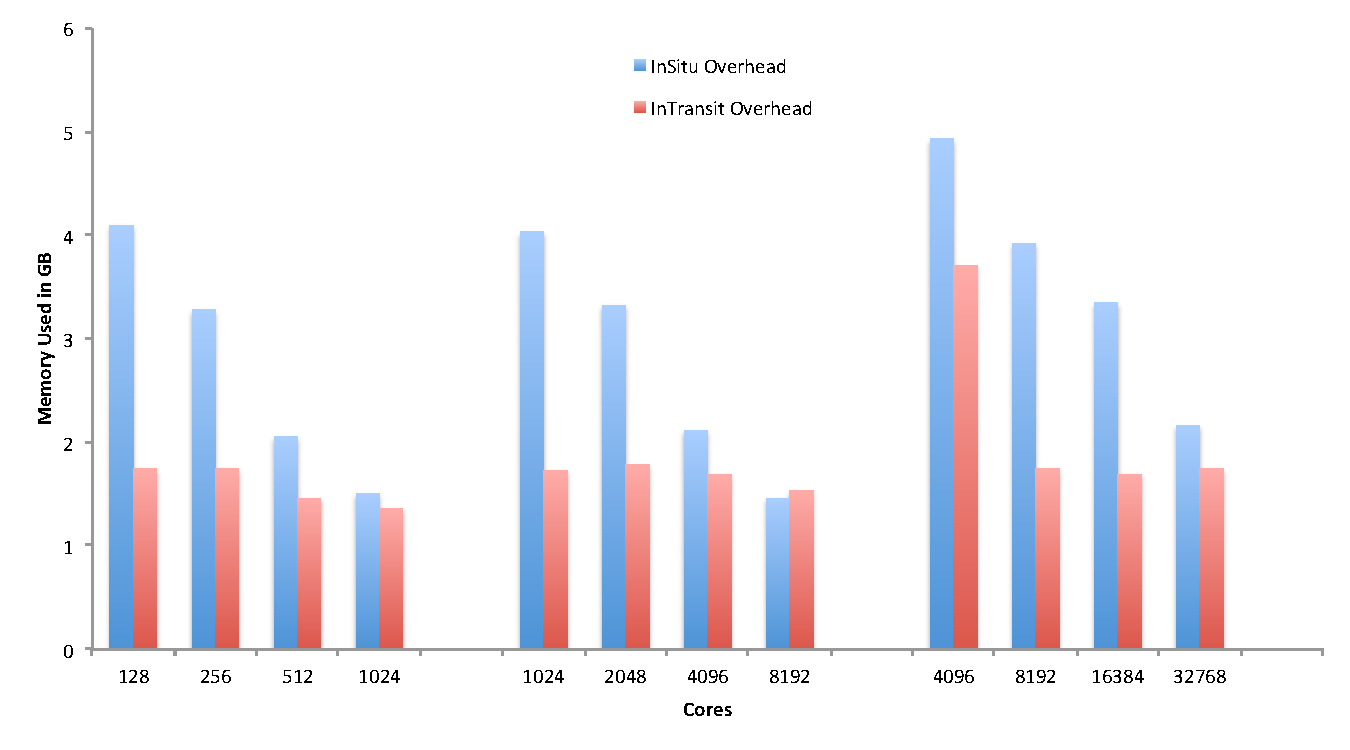
\includegraphics[width=\linewidth]{figures/MemoryUsageCompare.pdf}
  \caption{Plot of the average overhead per node of both InSitu and InTransit}
  \label{fig:MemoryCompare}
\end{figure}

\begin{figure}[htb]
  \centering
  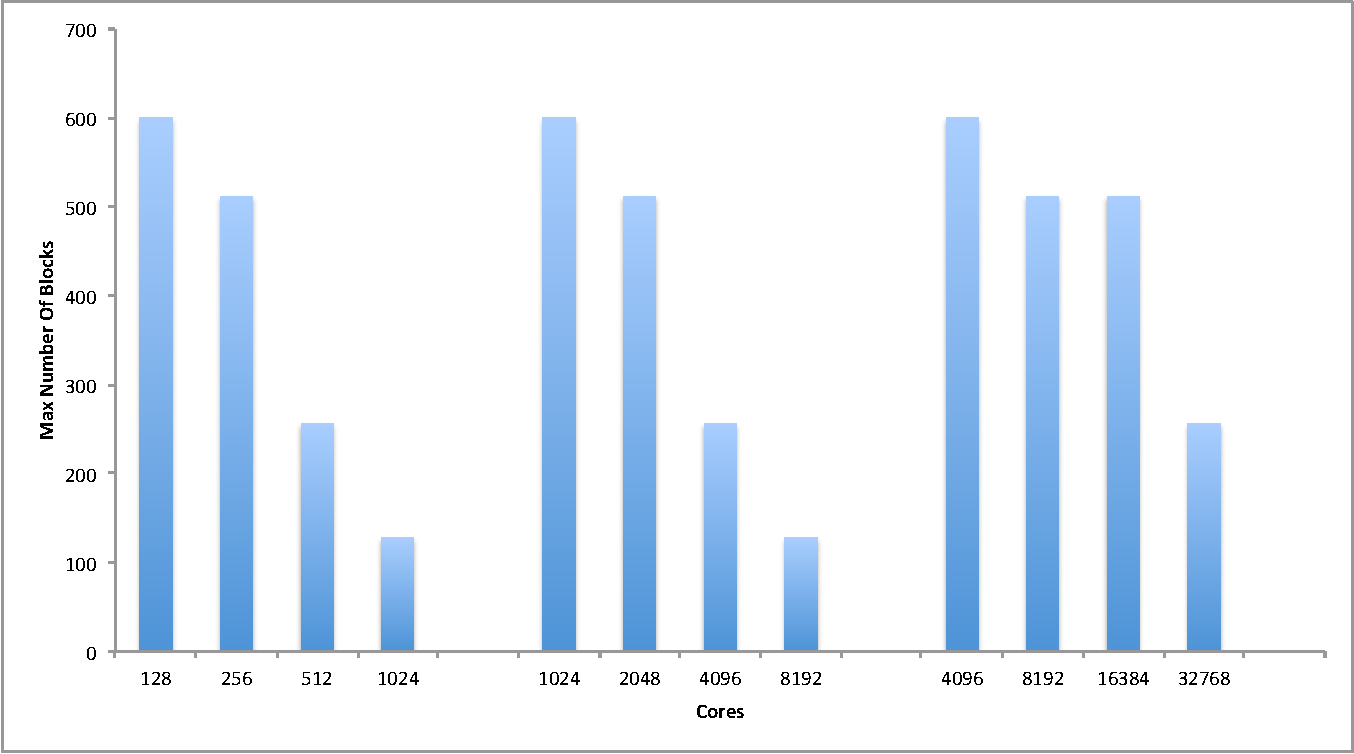
\includegraphics[width=\linewidth]{figures/MaxNumberOfBlocks.pdf}
  \caption{A plot of the "max number of blocks" parameter supplied to CTH for each run.}
  \label{fig:MaxBlocks}
\end{figure}


